\chapter{Quantum Computing and Quantum Homomorphic Encryption}
In this chapter we discuss what quantum computing and Quantum Homomorphic Encryption entails. 

\section{Quantum Computing}
In Quantum Computing, we have quantum bits (qubits) represented as $|0\rangle$ and $|1\rangle$  as opposed to the classical bits (0 or 1) in classical computing.  We also have quantum logic gates namely Hadamard (H), Z, X and CNOT which form the backbone of quantum computing. The gates can be represented as follows using circuit diagrams:
\begin{figure}[!h]
\center
\begin{minipage}[b]{0.3\textwidth}
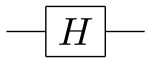
\includegraphics[scale=0.75]{images/hadamardgate.png} 
\caption{Hadamard gate}
\label{fig: Hadamard}
 \end{minipage}   
\hfill
\begin{minipage}[b]{0.5\textwidth}
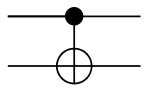
\includegraphics[scale=0.75]{images/cnotgate.png}  
\caption{CNOT gate}
\label{fig: CNOT}
\end{minipage}
\center
\begin{minipage}[b]{0.3\textwidth}
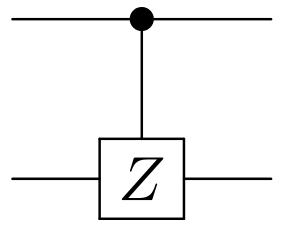
\includegraphics[scale=0.45]{images/zgate.png} 
\caption{Z gate}
\label{fig: Z}
 \end{minipage}   
\hfill
\begin{minipage}[b]{0.5\textwidth}
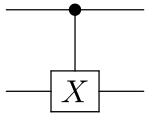
\includegraphics[scale=0.75]{images/Xgate.png} 
\caption{X gate}
\label{fig: X}
\end{minipage}
\end{figure}

The two main ideas brought about by quantum computing are superposition and entanglement which are adopted from quantum mechanics. If any computation uses these two mechanisms it is known as quantum computing. In quantum computing, a zero and a one can be represented simultaneously. This is known as superposition. It saves on processing time. For example, you have a box full of white chalks, but, you have one green chalk that you want to obtain from the box. The box is not transparent hence you cannot see what is inside. To solve the problem classically, you have to pull one chalk at a time until you get the green one. Quantum permits you to hold all the chalks at the same time and use probability to pull out the green chalk. This is the idea brought about by superposition.

Entanglement is when two particles interact and acquire states of each other, thus the output will be a mixture of the interacting particles, hence to describe one particle one has to refer to the other. To illustrate an entanglement, let us use a Hadamard and a CNOT gate. A CNOT gate is a Controlled NOT gate. If the control is a qubit of one then we apply a NOT to the bit in the target, otherwise nothing happens. This is shown in Figure \ref{fig:entanglement} below.

\begin{figure}[h]
\center
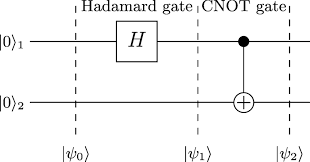
\includegraphics[scale=1]{images/entangle.png} 
\caption{An entangled circuit}
\label{fig:entanglement}
\end{figure}

At $|\psi_0 \rangle$ we have the output as $|0\rangle _1 |0\rangle _2$. It can also be written as $|0_1 0_2 \rangle$. We have $|0\rangle _1$ qubit passing through the Hadamard gate (H). By definition
$H|0\rangle =| \overline{0} \rangle = \dfrac{|0\rangle + |1\rangle}{\sqrt{2}}$. $|0\rangle _2$ does not change. The output $|\psi _1 \rangle $ is $ \bigg(\dfrac{|0\rangle + |1\rangle}{\sqrt{2}} \bigg)|0\rangle = \dfrac{|0\rangle_1 |0\rangle_2 + |1\rangle_1 |0\rangle _2}{\sqrt{2}}$. We then pass through the CNOT. Since $|0\rangle_1$ is 0, $|0\rangle_2$ remains unchanged, $|1\rangle_1$ is 1 hence $|0\rangle _2$ flips to $|1\rangle _2$. Thus the output $|\psi_2 \rangle $ is $\dfrac{|0\rangle_1 |0\rangle_2 + |1\rangle_1 |1\rangle _2}{\sqrt{2}} = \dfrac{|0_1 0_2\rangle + |1_1 1_2\rangle }{\sqrt{2}} = \dfrac{|0 0 \rangle + |1 1\rangle }{\sqrt{2}}$.

This is a maximally entangled state.

Quantum computing also supports parallelism. As opposed to classical computing where different processors are required, quantum computing parallelism is done on the same chip. As long as the tasks are related, they are carried out at the same time.

\section{Approach Techniques}
The properties of quantum computing enable computations to be performed on encrypted data (hidden).
This is the ability for a server to process data delegated to it, without accessing it. 
The two types of techniques used are Blind Quantum Computing and Quantum Homomorphic Encryption.
Blind actually means you cannot see. This encryption uses the same application. The server is blinded from input, output and computation. This is a technique where the server performs computations they do not know of on encrypted data and produces results which they do not also know from an encrypted input. Sounds hilarious right?
Quantum Homomorphic Encryption is a technique where the server performs computations they actually know of on encrypted data, that is, the input and output is encrypted but the computation is known.

\subsection{Differences between Blind Quantum Computing and Quantum Homomorphic Encryption}

\citep{broadbent2009universal}, \citep{fitzsimons2017private},\cite{ouyang2015quantum},\citep{Joe}

\begin{table}[!h]

\begin{tabular}{|c| c| c|}
\hline
 & Blind Quantum Computing & Quantum Homomorphic Encryption\\
\hline
1 & Everything is encrypted &   Only the input and output\\ 
 & (input, output and computation) &  are encrypted.\\
 &\citep{huang2017experimental} (abstract). &  \citep{broadbent2015quantum} (Introduction).\\
\hline
2 & Uses information theoretical security & Uses computational security protocol\\
  & protocol (can not be broken in) & (it is hard to break in).\\
  & \citep{fitzsimons2017private} (pg1).&  \\
\hline
3 & It is possible to expand the system & The system is fixed \\
& based on the client's needs &  \\
& \citep{Joe}.& \citep{Joe}.\\
\hline
4 & An interference with the protocol is usually & No measures are put into place hence there is a \\
  & detected because measures are put into place &  probability that an interference can go undetected.\\
  & \citep{broadbent2009universal}(abstract). & \\
\hline  
\end{tabular}
\caption{Differences between Blind Quantum Computing and Quantum Homomorphic Encryption }
\label{fig:table1}
\end{table}

\subsection{Why Choose Quantum Homomorphic Encryption Over Blind Quantum Computing?}

Information theoretical security used in Blind Quantum Computing is very hard to implement on a classical client hence its implementation is very expensive \citep{ouyang2015quantum}.  You cannot break into a system using information theoretical security even if your computational power is greater than the system. Due to the high cost  of implementation, very few clients will afford it. In most Blind Quantum Computing protocols, the client has some quantum computation requirements, though protocols that do not have this requirement exist \citep{broadbent2009universal}. This makes us choose Quantum Homomorphic Encryption which uses computational security which is hard to break in. Thus the risk of an adversary attacking the system is low.

\section{Quantum Homomorphic Encryption}
As seen earlier, it is possible to delegate tasks (data processing) to a server while the access to the data is not given away. The ability of a server to perform computations on encrypted data solves our security issue.  

\subsection{How the security issue is solved in Quantum Homomorphic Encryption?}


Since the server does not know the input or output it is impossible to change data to manipulate results, also, the integrity of the information is upheld. Data cannot be duplicated because, in quantum, duplication involves measurement and this changes the state thus you will never get the exact copy \citep{kassal2011simulating}. Quantum Homomorphic Encryption as we saw earlier, uses computational security. It is very hard to break or attack the encrypted data. To break in you require a lot of time. This makes it almost impossible for sensitive information to be leaked.


\subsection{How does Quantum Homomorphic Encryption work?}

There are four stages involved namely: Key generation, Encryption, Evaluation and Decryption \citep{broadbent2015quantum}.

All these stages are performed by the classical client . 

\subsection{Key generation and Encryption} 
Key generation produces a pair of public and private key. The public key is used to encrypt data while the private decrypts it. Key generation can be done using the RSA method. While using a computer program such as Python, an already existing RSA module exists. This implies that the client inputs a number and a pair of public and private key is generated. 

RSA can also be done using a mathematical approach. Two random large prime numbers say $p$ and $q$ are chosen. Let us take $p = 17$ and $q = 11$. We then calculate $N = p\times q$, $17\times 11 = 187$. $N$ is the system modulus.  The factorial of $p$ and $q$ is then calculated to find the public key which is used for encryption. In our example, we get the factorial as follows $(17-1)(11-1) = 16 \times 10 = 160 = 2^5 \times 5$. We now choose a number $e$ that does not divide any factor of $(p-1)(q-1)$. We can take our $e = 3$ as $3$ does not divide either $10$ or $16$. Thus $3$ is our public key. To get the private key we multiply our public key with a number say $d$ such that $ 1 = e \times d \mod (p-1)(q-1)$. We therefore calculate $d$ as follows, 
\begin{eqnarray*}
e \times d &\equiv & 1 \mod (p-1)(q-1)\\
3d &\equiv & 1 \mod 160\\
3d &=& 1 + k\cdot 160 \\
\end{eqnarray*}
$k$ is any random number that satisfies the equation. If we let $k =2$, then $d = 107$. Thus our private key is $107$ \citep{meissen2012mathematical}. Encrypted data can be referred to as a cipher text while unencrypted data is called a plain text. A plain text is transformed into a cipher text using the public key. Cipher text = (plain text)$^e \mod N$ while the plain text = (cipher text)$^d \mod N$.

The client can generate as many key pairs as they want to. This means that different public keys can encrypt the data producing different forms of encrypted data. The client is in a position to choose randomly which encryption to send. Since in homomorphic encryption the computation is known to the server, if you always send a certain encryption to perform the same computation, it would be easy for the server to start guessing. Also, if the server knows that different encryptions represent the same data, then it would be easy to guess too.

For example, you delegate the server to perform factorization. Factorization problems are easy to verify when given the results but hard to solve. It is very difficult for the server to know exactly which number you are factorizing since the input and output are encrypted. The computation does not reveal sufficient information about the input and output which would make an attack easy, apart from the input is a number and the outputs are prime numbers.

How many numbers and prime numbers exist? Will the server start guessing one by one? How long will it take for the server to actually guess the  correct number? It is possible for the server to guess the correct number but the probability is very low maybe 1 out of a million trials \citep{yang2013evaluation}.

\subsection{Evaluation and Decryption}
After key generation and encryption, we then evaluate. This is checking the correctness of the algorithm. The public key encrypts the already existing cipher text to produce another cipher text. For example let us encrypt \textit{g} in mod of a prime number say \textit{p}. Then we encrypt it again in$\mod 2$. Our cipher text reads c = (\textit{g} mod \textit{p}) mod 2. We first decrypt c in$\mod 2$ using the public key to check whether we will get \textit{g} mod \textit{p}. If we get the desired result then the algorithm is correct.  However the time taken to evaluate and the overall cost should be less than the individual cost of key generation, encryption and decryption. 

We have our cipher text and private key, we combine them to produce the plain text. Plain text = (cipher text)$^d \mod N$. This is our decryption process. The decryption  is done by the client after they receive the results of the delegated task \citep{ouyang2015quantum}.



